\section{Compound DMA attacks}\label{sec:linux_net}
\begin{figure}
    \centering
    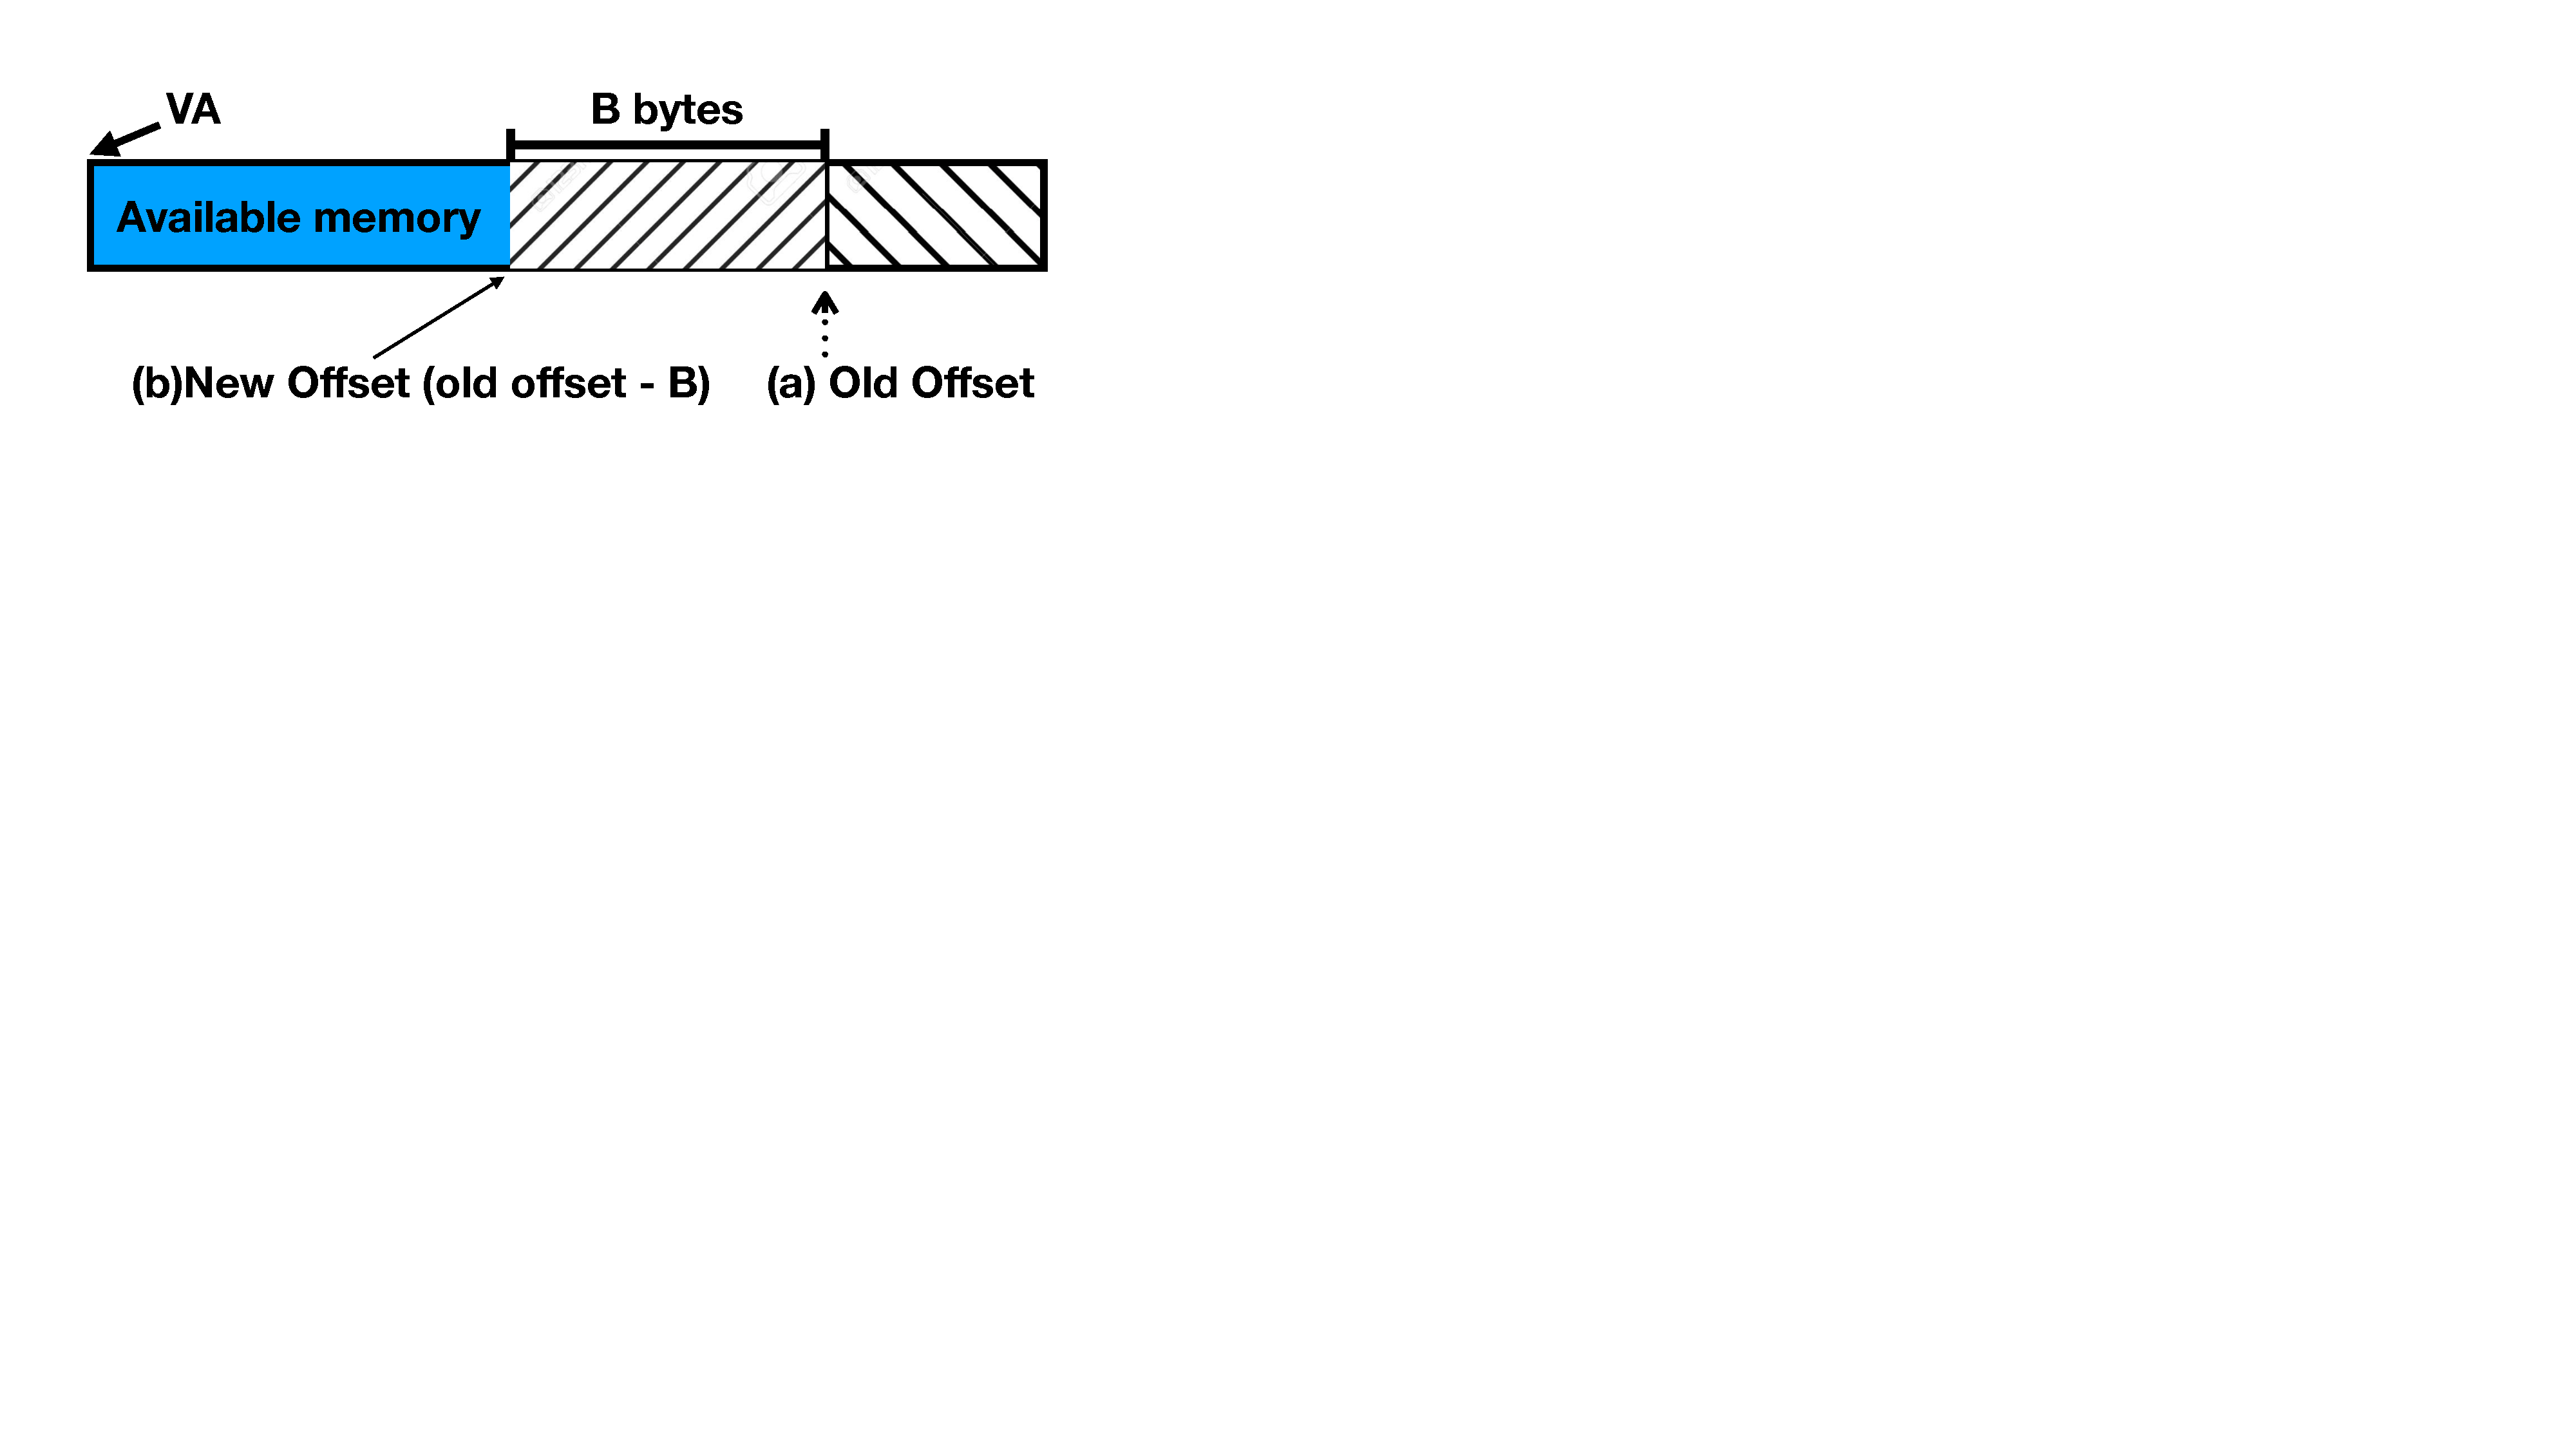
\includegraphics[width=1\linewidth]{figs/page_frag.pdf}
    \caption{Allocation of B bytes from page\_frag}
    \label{fig:page_frags}
\end{figure}

So far, we have discussed how a malicious device can take over a machine by exploiting type (a) sub page vulnerability of the FireWire driver. In this section we explore new attacks on the Linux network stack; where \means{} and \oportunity{} 
are initially missing but are attainable via compound steps, leaving room to dangerous privilege escalations attacks.

\subsection{\shinfo}
\begin{figure}[t]
    \centering
    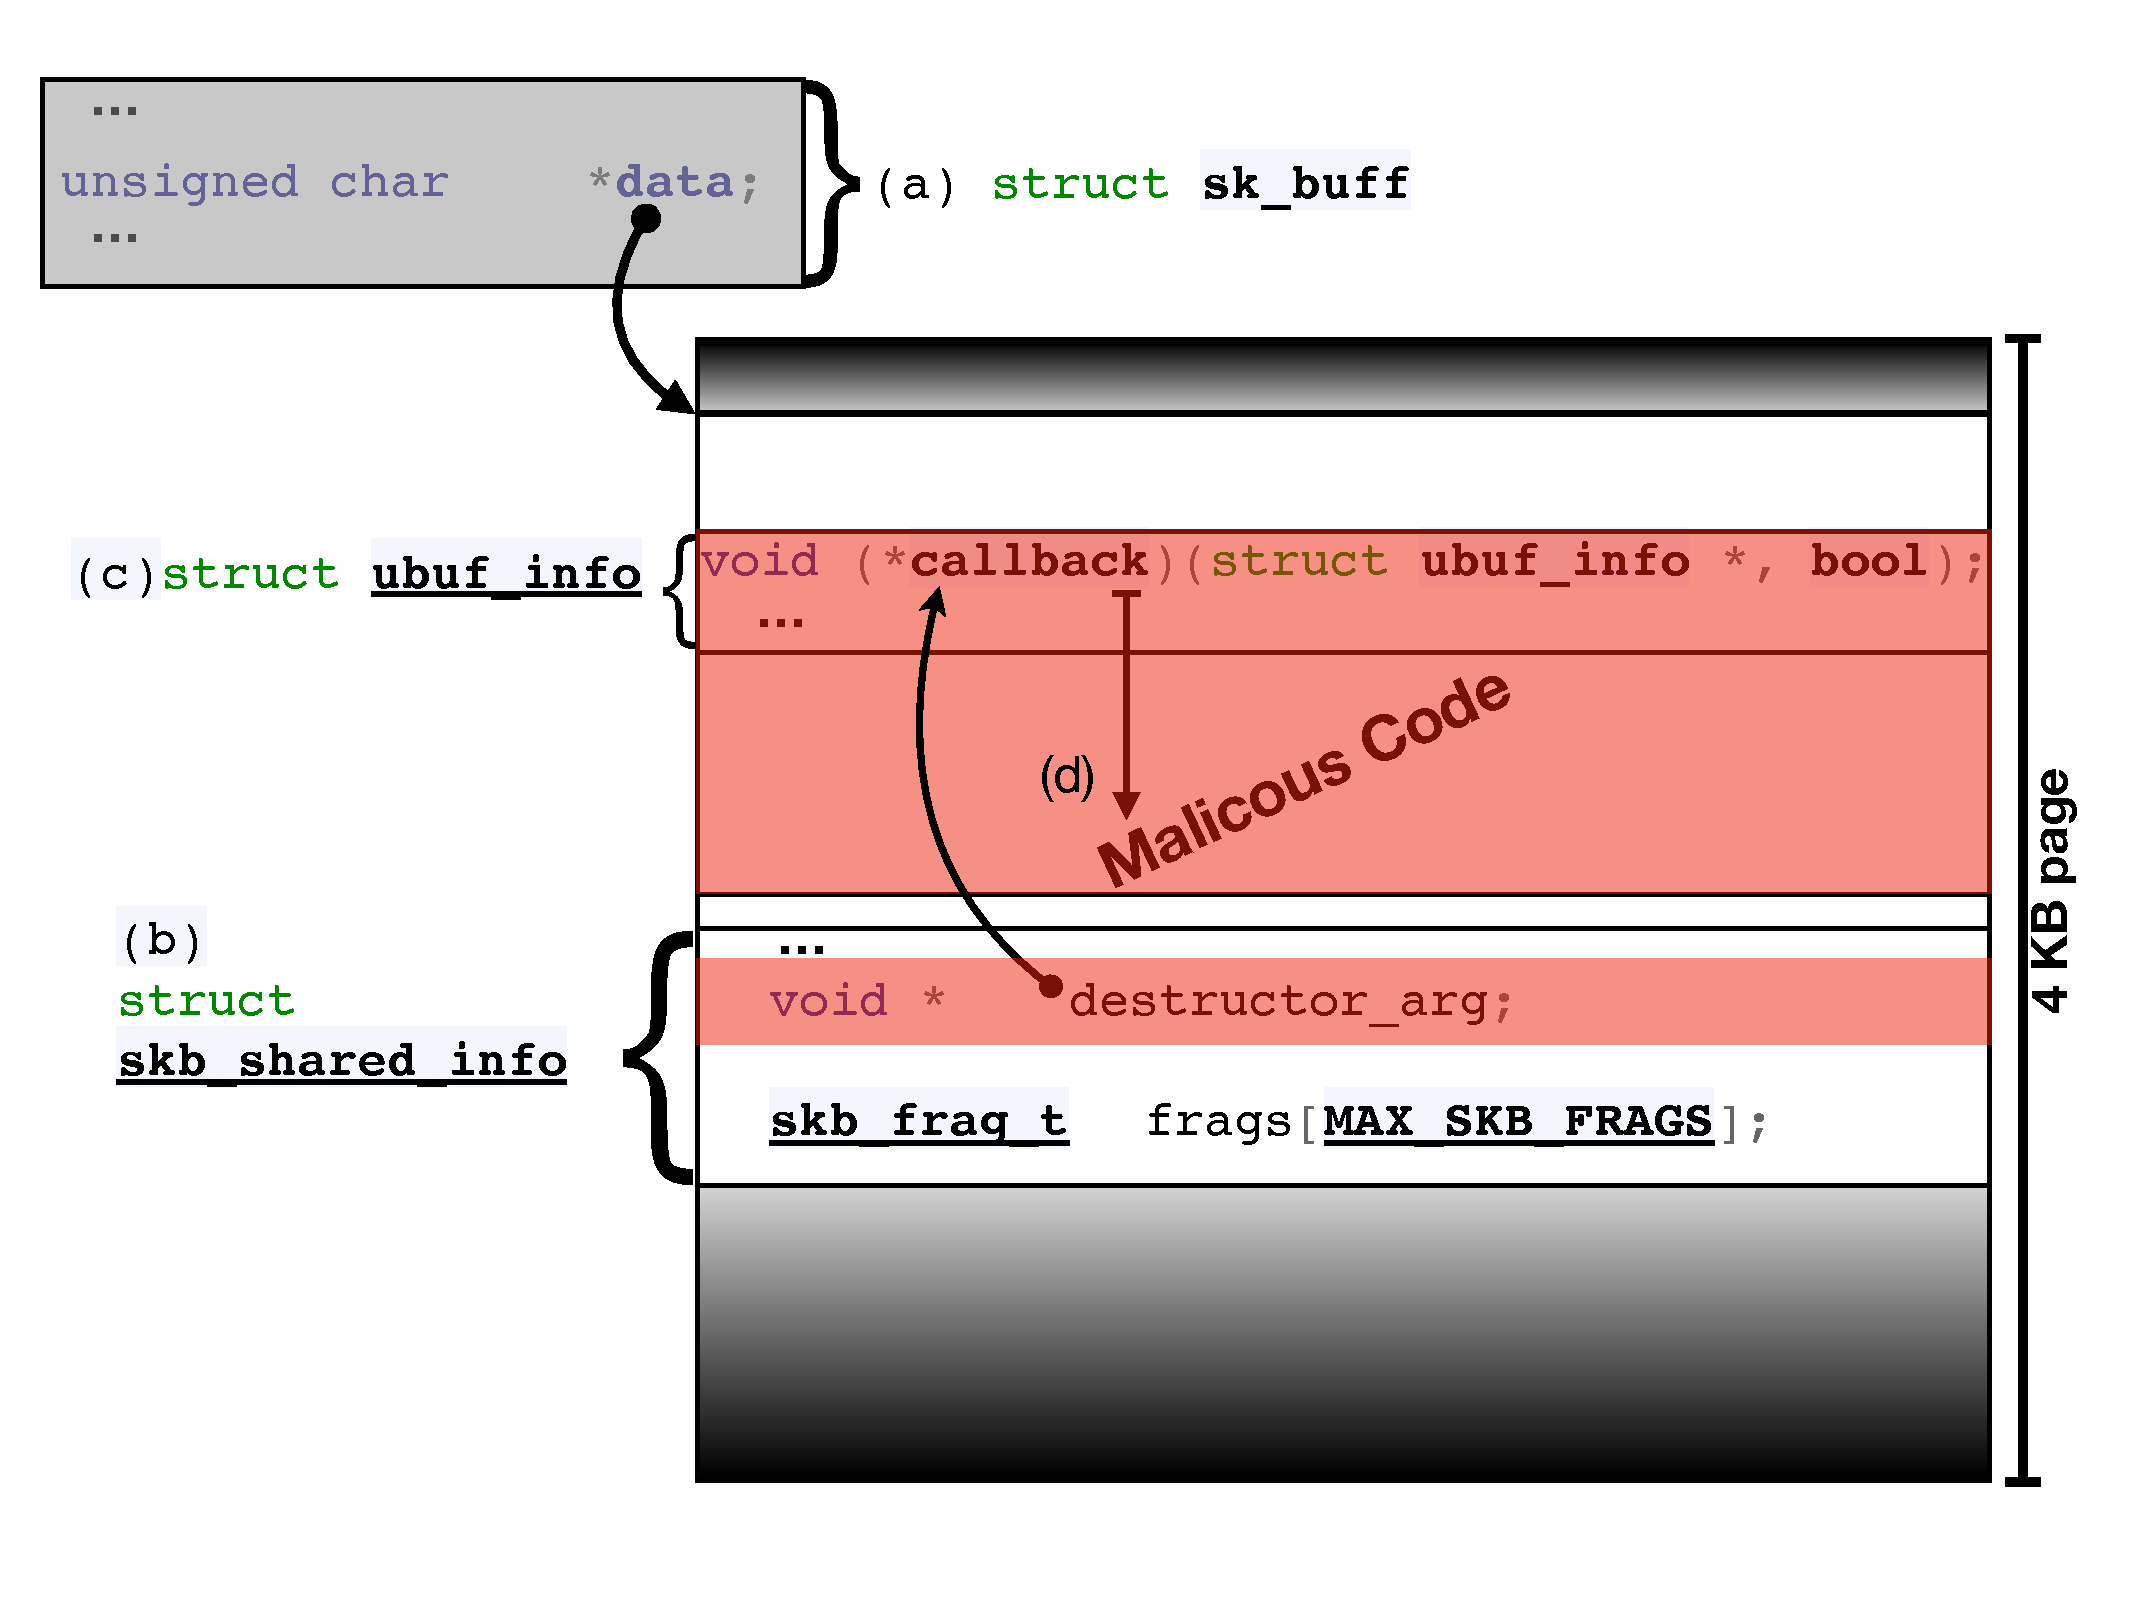
\includegraphics[width=\linewidth]{figs/ubuf.pdf}
    \caption{Using \shinfo{} to execute arbitrary code in kernel context.}
    \label{fig:sh_info}
\end{figure}

Struct \skb{} is a common data structure, used by the Linux network stack, to hold information representing a network packet. Struct \skb{} holds the metadata of a network packet (e.g., its size, associated socket). One of these fields is a pointer to a data buffer. The data is allocated separately, and thus, does not share a page with its \skb{} (Fig. \ref{fig:sh_info}). 

This separation means that \skb{} is \emph{never} (intentionally) mapped to the device. Indeed, it is a common belief, pointed out in literature \cite{thunder}, that the Linux network stack is not susceptible to DMA attacks via the \texttt{data} pointer. In this work, we show that this belief is misplaced.

The Linux network stack supports packet cloning by merely copying \skb{} metadata. This includes the \texttt{data} pointer. That is, the resulting \skb{} and the original one share the data buffer \cite{drivers2005linux}. Note that the data buffer of the \skb{} is the \emph{linear} part of the payload but \skb{} also supports \emph{non-linear} buffers, ferrying payloads in page fragments (i.e., buffers described by their \page{}, length and offset). 

To support these non-linear buffers, the \shinfo{} metadata structure is used.
Struct \shinfo{}, in contrast to \skb{}, is always allocated as part of the data buffer. Therefore it is always mapped to the device. \shinfo is unwittingly mapped with the permissions of the packet, i.e., WRITE for RX packets, READ for TX packets, and in some cases, such as XDP/XSK \cite{xdp} with BIDIRECTIONAL.

Consequentially, \shinfo{} is the potential \oportunity{} the malicious device has been looking for. The sub page vulnerability created by \shinfo{}, represents a type (b) vulnerability (Fig. \ref{fig:colocation} (b)), as this is innate to Linux networking rather than a driver security bug. 

Fig. \ref{fig:sh_info} depicts how a malicious device can mount an attack using \shinfo{} in four steps:
\begin{enumerate}[label=(\alph*)]
    \item An RX \skb{} and its data buffer are allocated. The data buffer is mapped for the NIC with WRITE access (the WRITE access is to the whole 4~KB page). 
    \item \texttt{destructor\_arg} field in \shinfo{} is overwritten to point within the mapped page. Now, the \texttt{destructor\_arg} is pointing to struct \uarg{} which is created by the NIC.
    \item \uarg{} has a callback pointer that is now pointing to the malicious code that resides on the same page. In the case of NX-bit, it is a poisoned ROP stack.
    \item when the \skb{} is released, the callback is invoked.
\end{enumerate}
To expand this scenario into a complete attack, the attacker must complete the MMO trifecta. That is, both \means{} and \oportunity{} are required. \textcolor{olive}{In the next subsection, we demonstrate how an attacker can leverage the standard OS behavior to find the missing attributes.}

\subsection{Hacking~\oportunity{}}\label{sec:shinfo}

\begin{figure}[t]
    \centering
    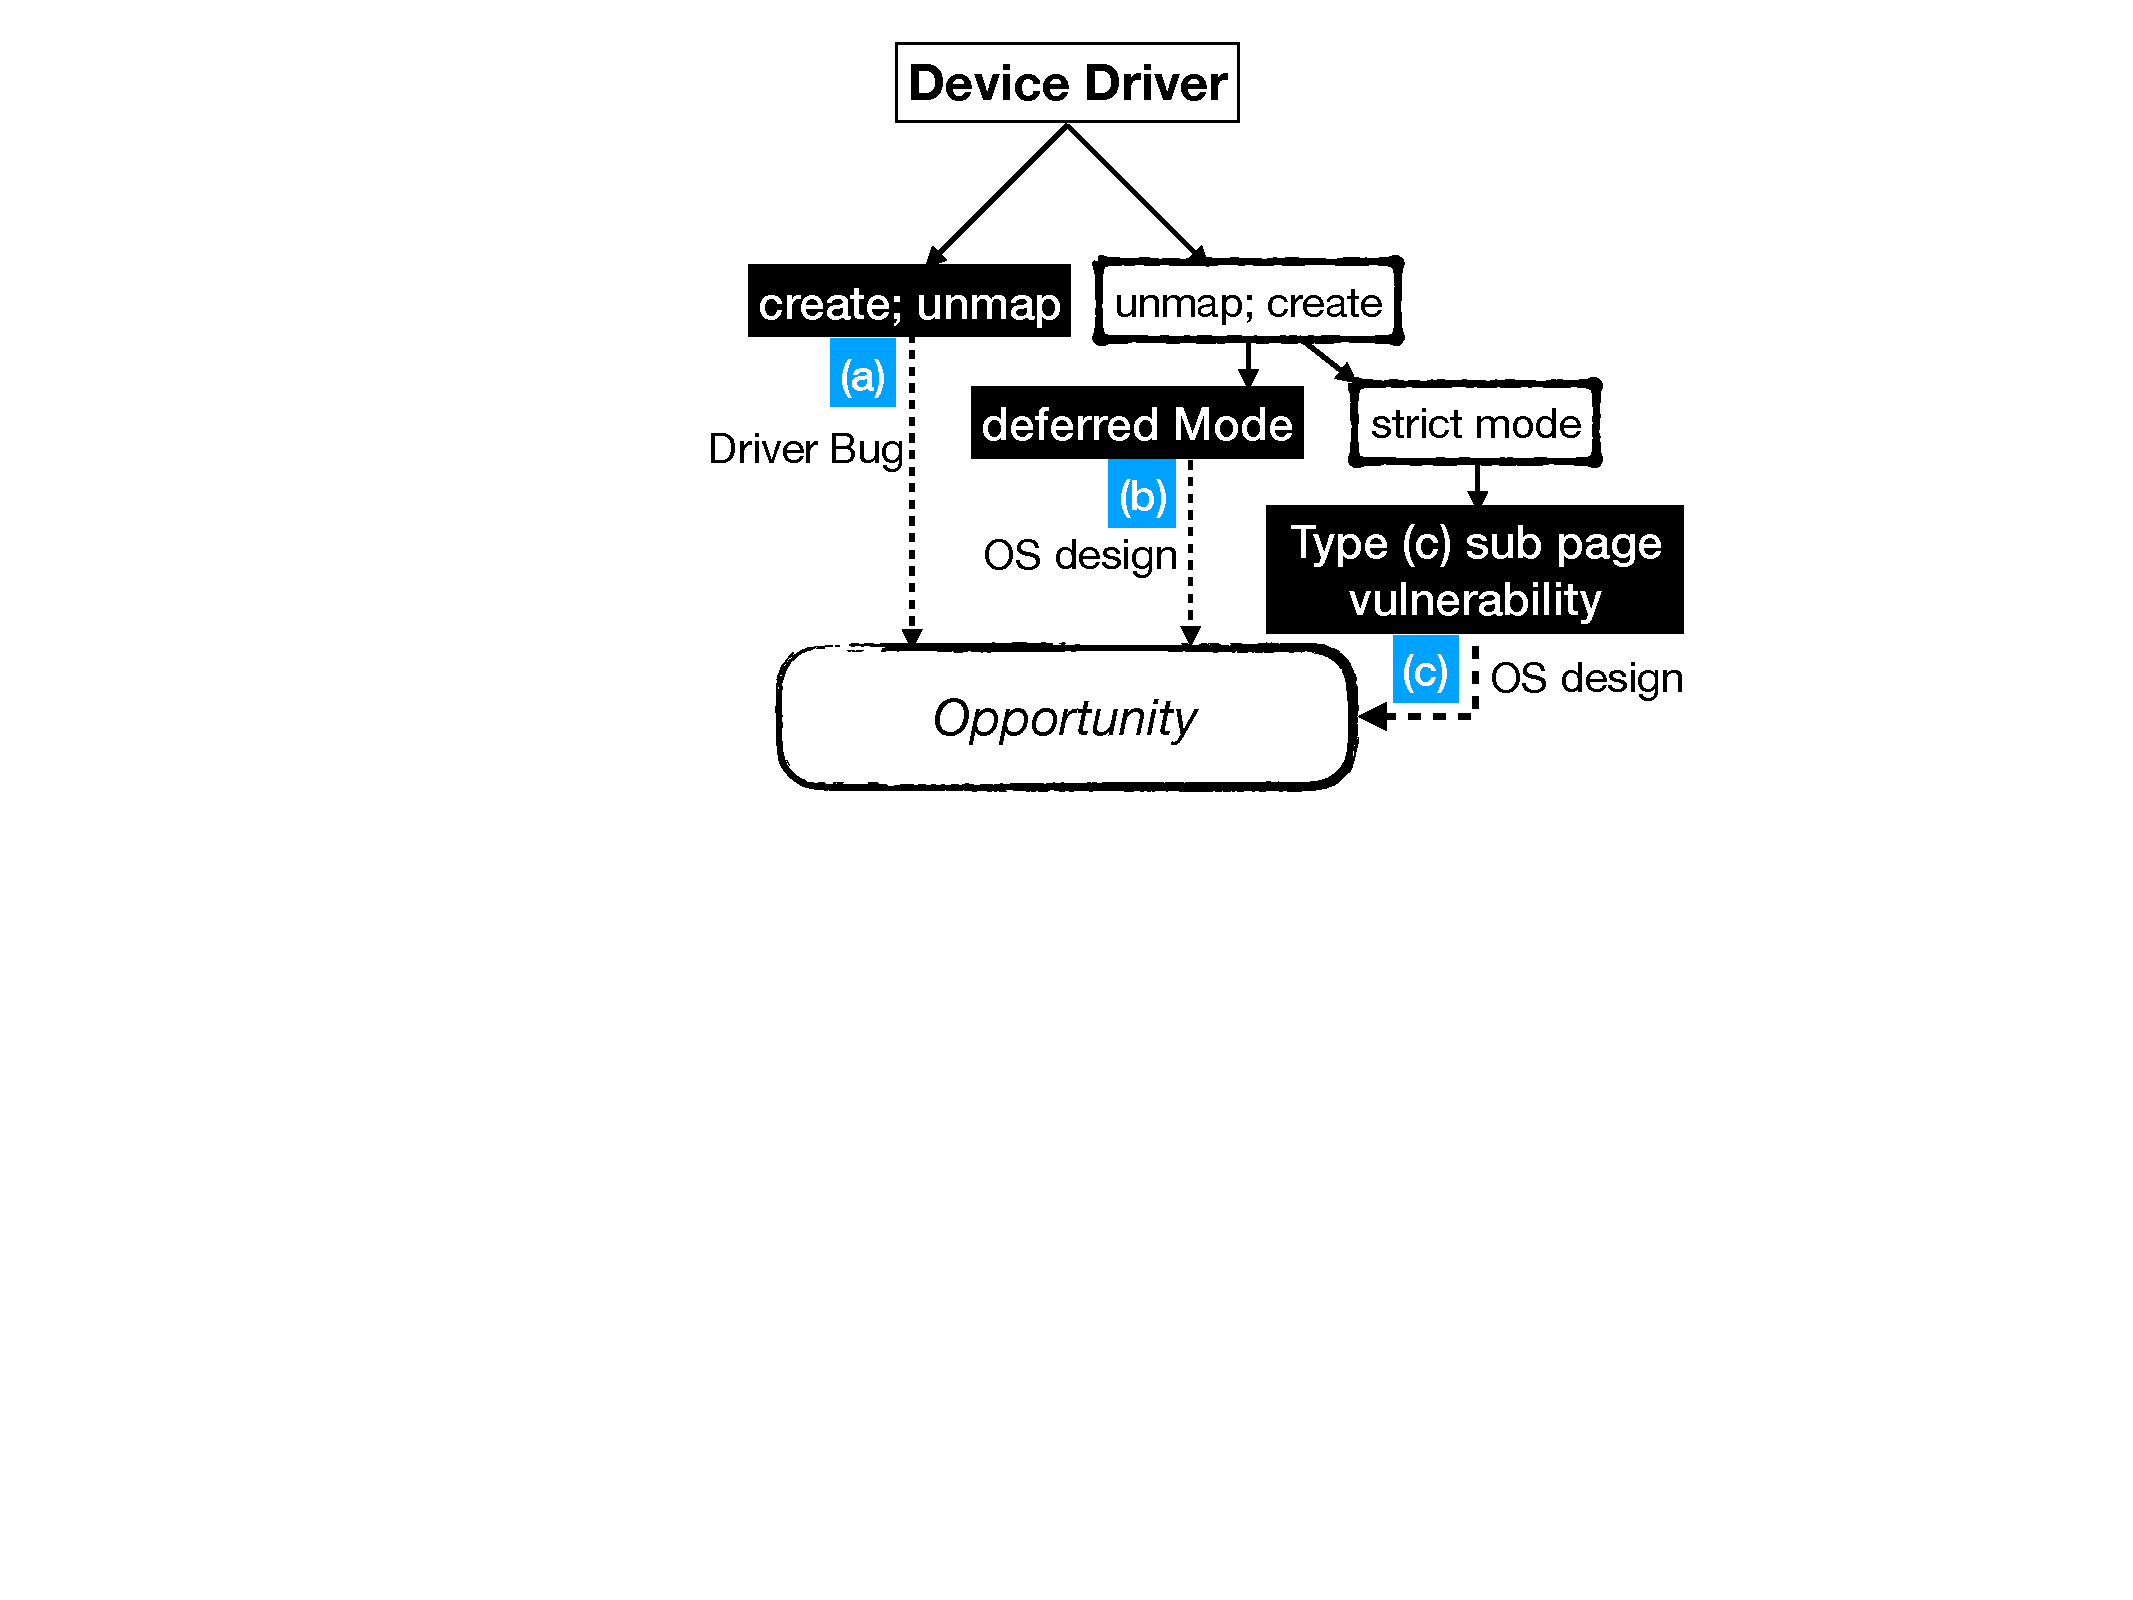
\includegraphics[width=\linewidth]{figs/road_to_op.pdf}
    \caption{Different ways to obtain \oportunity.}
    \label{fig:road_to_op}
\end{figure}

As depicted in Fig. \ref{fig:road_to_op}, we now details different ways ((a), (b) and (c)) in which a malicious device obtains \oportunity{}.

\begin{enumerate}[label=(\alph*)]

\item Presumably, a correct use of the DMA API should thwart the attack outlined in the previous section (Fig. \ref{fig:sh_info}). Namely, unmapping the buffer and only then initializing \shinfo{} should allow the CPU to undo any malicious changes the NIC may have perpetrated. 
As it turns out, prevalent device drivers (Appendix \ref{apndx:wrong_order}) first create an \skb{} and only then unmap the buffer. This order of execution allows the \emph{device} to undo legitimate changes to \shinfo{} by the CPU. 

\item Nevertheless, even when the order is correct, i.e., the unmapping of the buffer occurs before the creation of the \skb{}, still \shinfo{} is not safe from later modifications. As the default IOMMU mode in Linux is \emph{deferred} protection (Sec. \ref{sec:deferred}), the umap order is made irrelevant. That is, even though the unmap function is invoked in the correct order, the device can still corrupt \shinfo{} due to the IOTLB. Namely, the device can control which \iova{} are cached in the IOTLB by accessing only the addresses it needs cached. 

\item In response, a security-conscious admin may change the default setting to \emph{strict} mode, where the IOTLB is flushed on every unmap. However, this both severely degrades networking performance \cite{MMT16,MSMT18}, and does not alleviate the security threats on the system. Presumably, with \emph{strict} mode enabled, the \iova{} the NIC used to access that \shinfo{} is no longer valid, which initially sounds promising. The problem is that the device, in many cases, will still have legitimate WRITE access to the physical page of the \shinfo. The vulnerability stems from the way \data{} is allocated. An RX \skb{} is almost exclusively allocated via an API (e.g., \texttt{napi\_alloc\_skb} or \texttt{netdev\_alloc\_skb}) that creates a type (c) sub page vulnerability (Fig. \ref{fig:colocation} (c)). The device can use the \iova{} of a co-located buffer to access the \shinfo{} it requires. Particularly, the buffers of the driver RX ring are allocated sequentially, resulting in pairs of successive RX descriptors that map the same page. Obviously, this holds as long as the buffer sizes are smaller than 4 KB. This is a reasonable assumption since the default MTU size is 1500~B. These allocation functions, use a \texttt{page\_frag} mechanism to allocate the \data{} buffers, which in turn contain \shinfo. The \texttt{page\_frag} is an efficient method for allocating small buffers, often used by the Linux network stack. A \texttt{page\_frag} is initialized by allocating a contiguous memory region (usually 32 KB), setting a \textit{va} pointer to the beginning of the region and \texttt{offset} to the end. An allocation request for \texttt{B} bytes subtracts \texttt{B} bytes from the \texttt{offset} pointer and returns the new value of \texttt{offset}\footnote{In multicore environments, the \texttt{page\_frag} uses a different buffer for each CPU and each CPU has a single RX ring. As a result, each RX ring is served by its own (per-CPU) contiguous buffer.} (Fig. \ref{fig:page_frags}). This mechanism for memory allocation is efficient, but results in consecutive \data{} buffers sharing memory pages. Due to this type (c) sub page vulnerability, the NIC does not require the invalidated \iova{} to modify the \shinfo; instead, it can use the \iova{} for the next data buffer. Note that the lower 12 bits (the offset on the page) of the \iova{} are identical to the corresponding \kva{} bits. As illustrated in Fig. \ref{fig:sh_info}, the \oportunity{} obtained is via the next buffer (i.e., the striped area at the end of the page).
\end{enumerate}

\textcolor{olive}{
The drivers on our setup, namely bnx2 and mlx5\_core are both vulnerable. The bnx2 driver uses the correct unmapping order, and uses kmalloc to allocate its RX buffers, instead of the dedicated API functions (e.g., \texttt{napi\_alloc\_skb} or \texttt{netdev\_alloc\_skb}), but due to \emph{deferred} mode, \shinfo{} is still vulnerable to modifications.
The mlx5\_core driver, avoids unmapping the RX buffers altogether, in kernel 5.0, the driver uses a \texttt{pool\_page} mechanism\cite{page_pool} and in kernel 4.15, the driver uses an ad-hoc mechanism, to achieve the same goal as \texttt{pool\_page}. These, design choices, in both cases leave \shinfo{} vulnerable, both in \emph{deferred} and \emph{strict} modes.  
The discrepancy in driver behavior, is due to the fact that bnx2 is a driver for a 1 GBE NIC; where as, mlx5\_core is a 50 GBE\footnote{\textcolor{red}{Ours is an x8 model rather than the x16, that can reach 100GB/s.}}, and uses more efficient APIs to maximise performance.}



\smallskip
Interestingly, as it stands today, it seems that the only way to secure \shinfo{} is to never map it. 


\smallskip
\textcolor{olive}{From this point on, we assume that the attacker has unimpeded access to \oportunity{}. In the next subsections, we demonstrate various compound DMA attacks where an attacker can exploit OS behaviour to gain \means{} and \motivation{} completing the trifecta.}

\subsection{Ring Flod}\label{sec:ringflod}

A malicious device can generate a poisoned ROP stack on each RX buffer and gain \motivation{}. At this point, the device still cannot execute a successful code injection attack; the device is lacking \means{}. 

Due to the IOMMU, the device has all the \iova{} for the RX buffers, but not the \kva{}. In this attack we take advantage of the fact that the boot process is \emph{deterministic}. Each reboot, the same set of commands is executed in the same order initiating the same kernel modules and starting the same processes. While the actual pages each module gets vary in a multi-core machine due to timing issues, the drift is not expected to be too large.

We evaluate this assumption also on a DELL 730 server equipped with a ConnectX-4 NIC, running 256 reboots on Ubuntu 18.04 with kernel 5.0. 
\footnote{\textcolor{red}{Please generate table of RingFlod Results}}

We find that many of the PFNs repeat in more than 50\% percent of reboots. \footnote{\textcolor{magenta}{Need to see If we can improve this number}} Thus an adversary with knowledge about the physical setup can guess with a high probability a valid \kva{} for one of the RX pages. Now with a valid \kva{} for a \mabaf{},  i.e., \means{} and \motivation{}, the trifecta is complete and the attacker is able to execute the attack as shown in Fig. \ref{fig:sh_info} (in this case the \texttt{destructor\_arg} will most likely indicate a different page, but other that the attack scenario is unchanged).

The success probability of this attack depends on the driver version and NIC capabilities. For example ,some NICs have a HW LRO capability; where a NIC can aggregate multiple TCP packets into a single TCP packet, larger than MTU \cite{mlx5_lro}(e.g., bnx2x, mlx5\_core). On drivers configured with these options each RX buffer is 64KB regardless of MTU. As a result, these drivers have a much larger memory footprint\cite{MSMT18} and are much easier to target with a RingFlod attack.

\begin{figure*}[t]
    \centering
    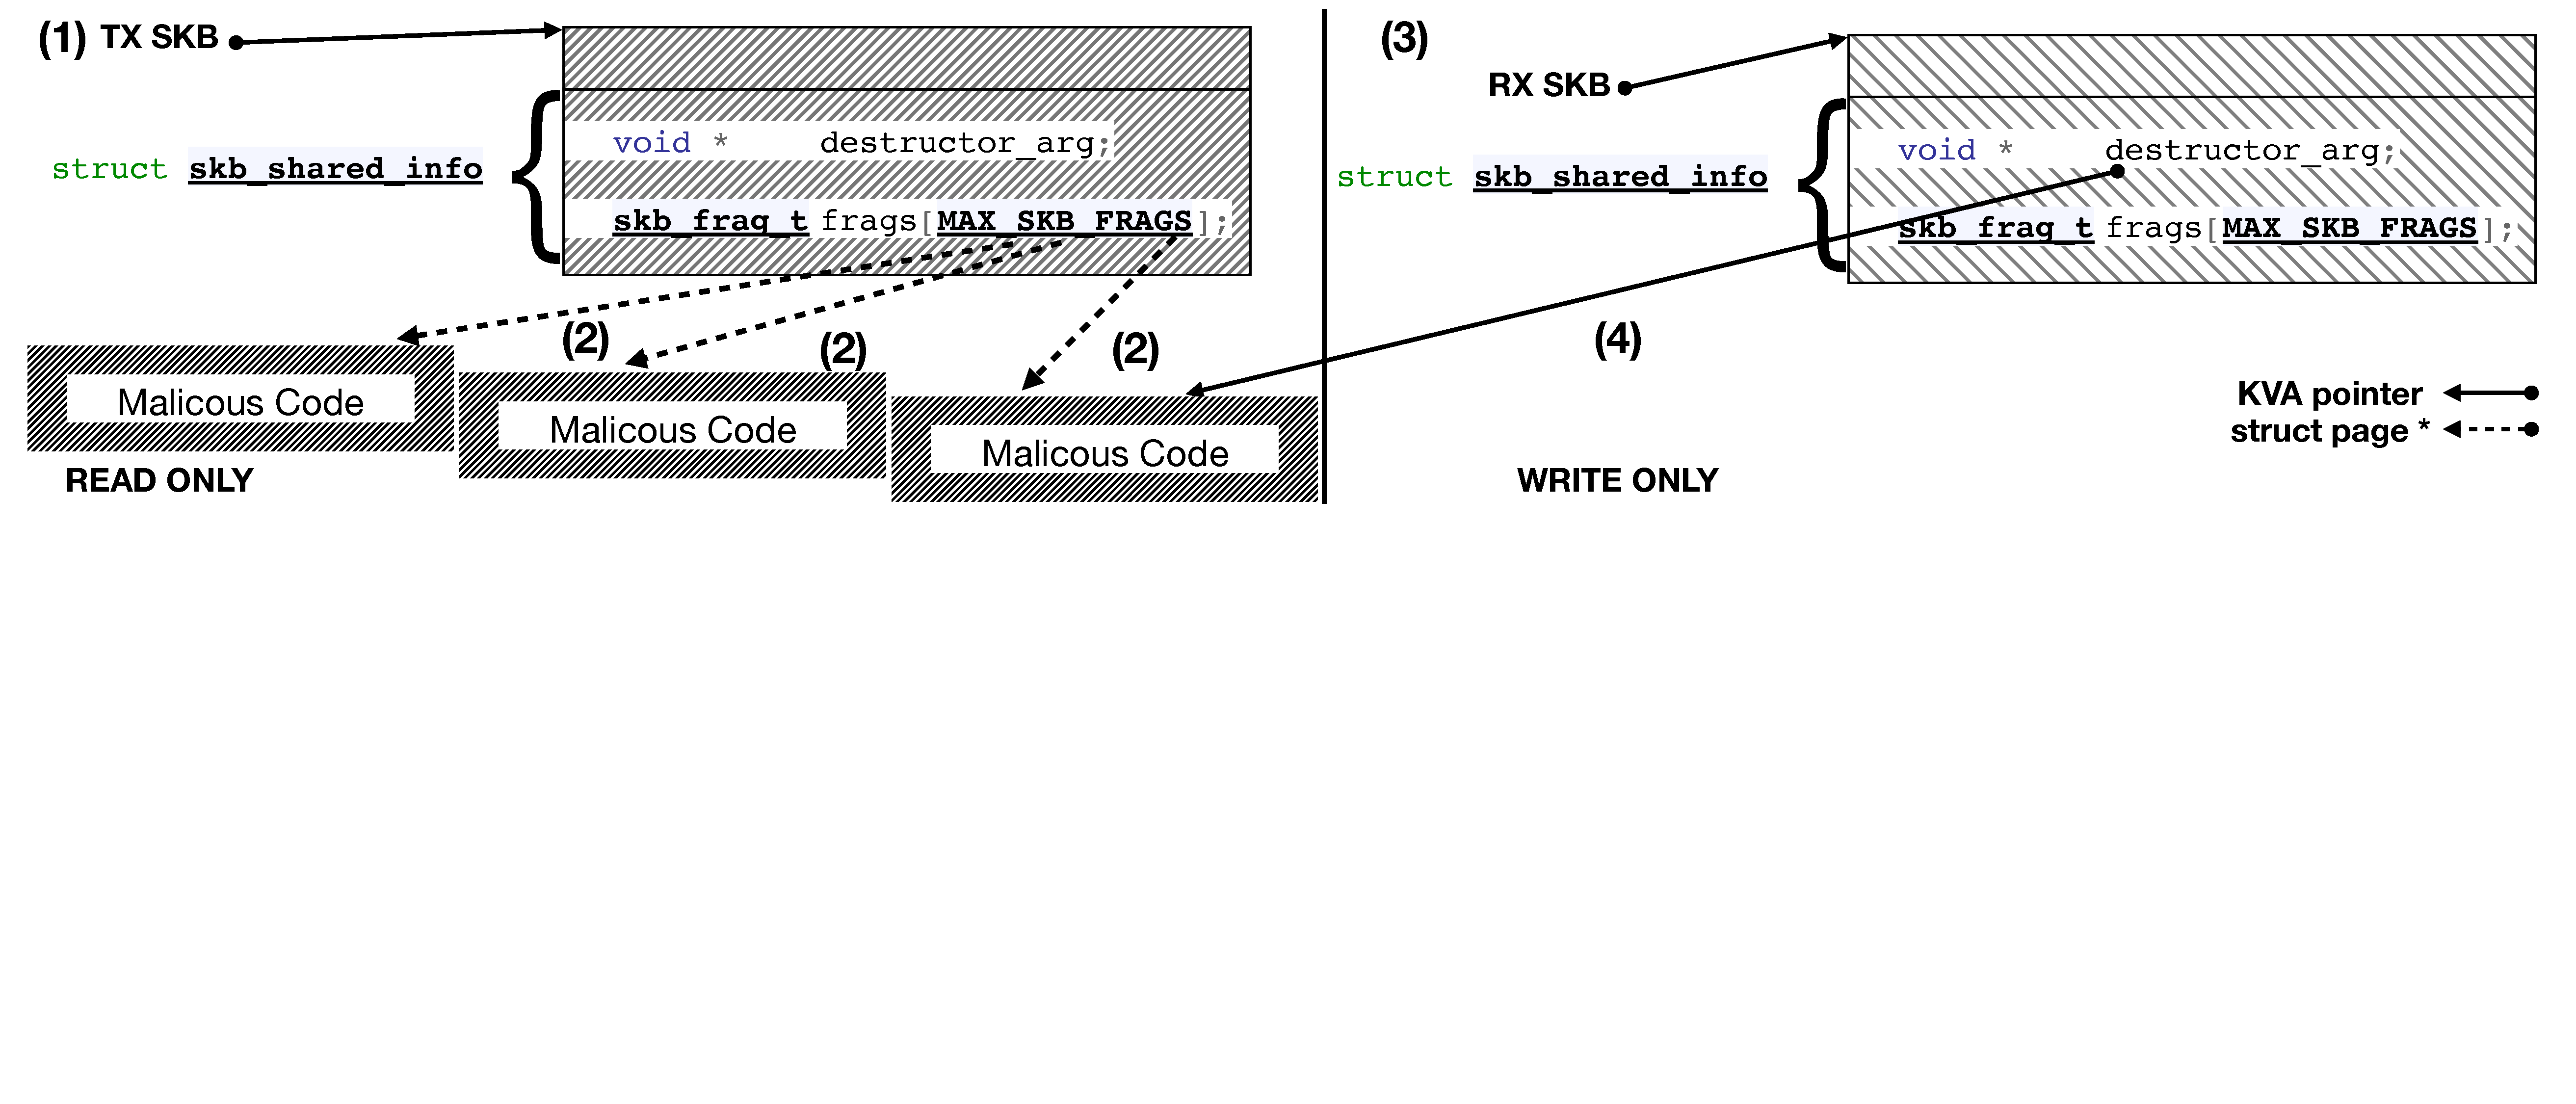
\includegraphics[width=\linewidth]{figs/accomplice.pdf}
    \caption{A TX sk\_buff filled with malicious code, used as a \means for a DMA attack}
    \label{fig:payload}
\end{figure*}
\subsection{Poisoned TX}\label{sec:posion}

\textcolor{magenta}{RingFlod \ref{sec:ringflod} allows a NIC to execute random code with high probability. The prerequisite, is enough information regarding the physical layout of the server and its peripherals\footnote{Other PCIe devices and their location, this all impacts how memory is allocated} and as long as the NIC driver has a high enough memory footprint. }

When guessing a \emph{magic} PFN is not an option, we need other \means of computing a valid \kva. 
A NIC has READ access to the \shinfo of a TX packet, this provides the NIC with access to the frags array. The \texttt{frag} array contains struct \page{} pointers, that both leak kernel pointers that allow to break KASLR, and provide the PFNs of specific pages containing data sent from userspace; pages that device can access with READ. 

Assuming, an unprivileged accomplice(witing or unwitting) can open a UDP/TCP socket in user space; this user could transmit a poisoned ROP buffer. 
%For a ROP attack (where we need the Kernel text offsets) we assume the NIC has spoofed an UDP packet with poisoned content for the accomplice to send. 
Once an accomplice sends the packet the NIC can execute the attack in 4 simple steps (Fig \ref{fig:payload}):
\begin{enumerate}
    \item The TX \data and the fragments are mapped for the NIC to read.
    \item The NIC identifies the poisoned buffer and translates \page to \kva.
    \item The NIC spoofs an RX packet, and delays the completion notification of the TX packets (we don't want the \mabaf to be released prematurely).
    \item The NIC overwrites \shinfo with the \kva retrieved in step 2. 
\end{enumerate}
%But if the fragments hold malicious content; its all the malicious NIC needs for a successful attack. The readable \shinfo holds a \kva for a \page. This both allows the NIC to break KASLR and gives a \kva\footnote{\textcolor{magenta}{Do show exactly what are the KASLR bits and how you break it}} of a valid \mabaf. To implement the attack the NIC will generate an RX packet and fill the \uarg address from the calculated \kva.
%The NIC will hold off on the TX completion event in order to make sure that \kva is not freed by the TX completion handler; before the poisoned RX packet is processed. A TX completion event that fails to appear in due time, will trigger a TX T/O error that will flush all buffers; the T/O is set by the driver usually to 5 seconds, which is enough to implement an attack.\newline
In this scenario the attacker doesn't need any prior knowledge of the kernel or the hardware. The only assumption is that there is an accomplice (witting or unwitting) that can open a socket in user-space. For that matter, a socket in user-space of a guest machine; making any cloud VM or a Proxy server a valid intrusion tool in the presence of a malicious device.\newline
Having an accomplice, in the form of an unprivileged user provides other vectors of attack as well. In addition to running ROP attacks; the NIC can also leak the content of arbitrary memory pages to the user. Assuming that the NIC has write access to \shinfo after it has been sent up the network stack. For example, in case of deferred protection or when pool\_page is used (see \ref{sec:xdp}). The NIC can modify the \page address in the \texttt{frag} entries, and let the Linux network stack copy the context of arbitrary memory pages to an unprivileged user. A likely side effect of this attack is a memory corruption and a Kernel panic; so caution is advised. The reason beaing, that the \texttt{skb\_free} function will attempt to free these pages; pages never owned by the network stack.
\newline
\textcolor{magenta}{Must validate feasibility: An accomplice in user space, can attempt running arbitrary code in kernel context without resolving to ROP attacks; the usef, can instead write a function and a \texttt{ubuf\_info} in an unprivileged binary and send the \texttt{ubuf\_info} address to the NIC. The \shinfo callback must be called with the users page tables loaded - this is a likely scenario as it seems that the \skb is freed inside the recv() sys\_call callback.}

\subsection{Forward Thinking}
In some situations, an accomplice will not be available. Packet forwarding functionality is usually disabled by default in Linux machines. But some Linux servers may function as a router or an L3 load balancer; these machines will have packet forwarding enabled. In this scenario instead of waiting for an accomplice to send a poisoned packet; the NIC can independently generate an RX packet to a destination that is reachable from the server. For a TCP connection, the Linux kernel will attempt to aggregate multiple TCP segments into a single large packet\footnote{Generic Receive offload,\url{https://access.redhat.com/documentation/en-us/red_hat_enterprise_linux/6/html/performance_tuning_guide/network-nic-offloads}}. This packet will then be forwarded and become a TX packet. A TX packet that can be used as described in the previous attack (\ref{sec:posion}) Fig \ref{fig:payload}. \newline
Packet forwarding, also opens up additional attack options. Instead of sending a TCP packet and letting the GRO layer fill in the \texttt{frags} information. The NIC can generate a small UDP packet and fill in the \texttt{frags} array with any arbitrary \page on the system. This will make the driver map these pages with DMA\_TO\_DEVICE; providing read access to any page on the system to the NIC. The ConnectX-5 driver (mlx5\_core), will map all the frags in \shinfo, w/o checking the actual packet length. It is important to set the \texttt{nr\_frags} field to let the driver know that there are frgas to map. But setting the field back to zero, before creating a TX completion. It is important, that the OS wont try freeing pages the driver never owned.

\begin{figure*}[t]
    \centering
    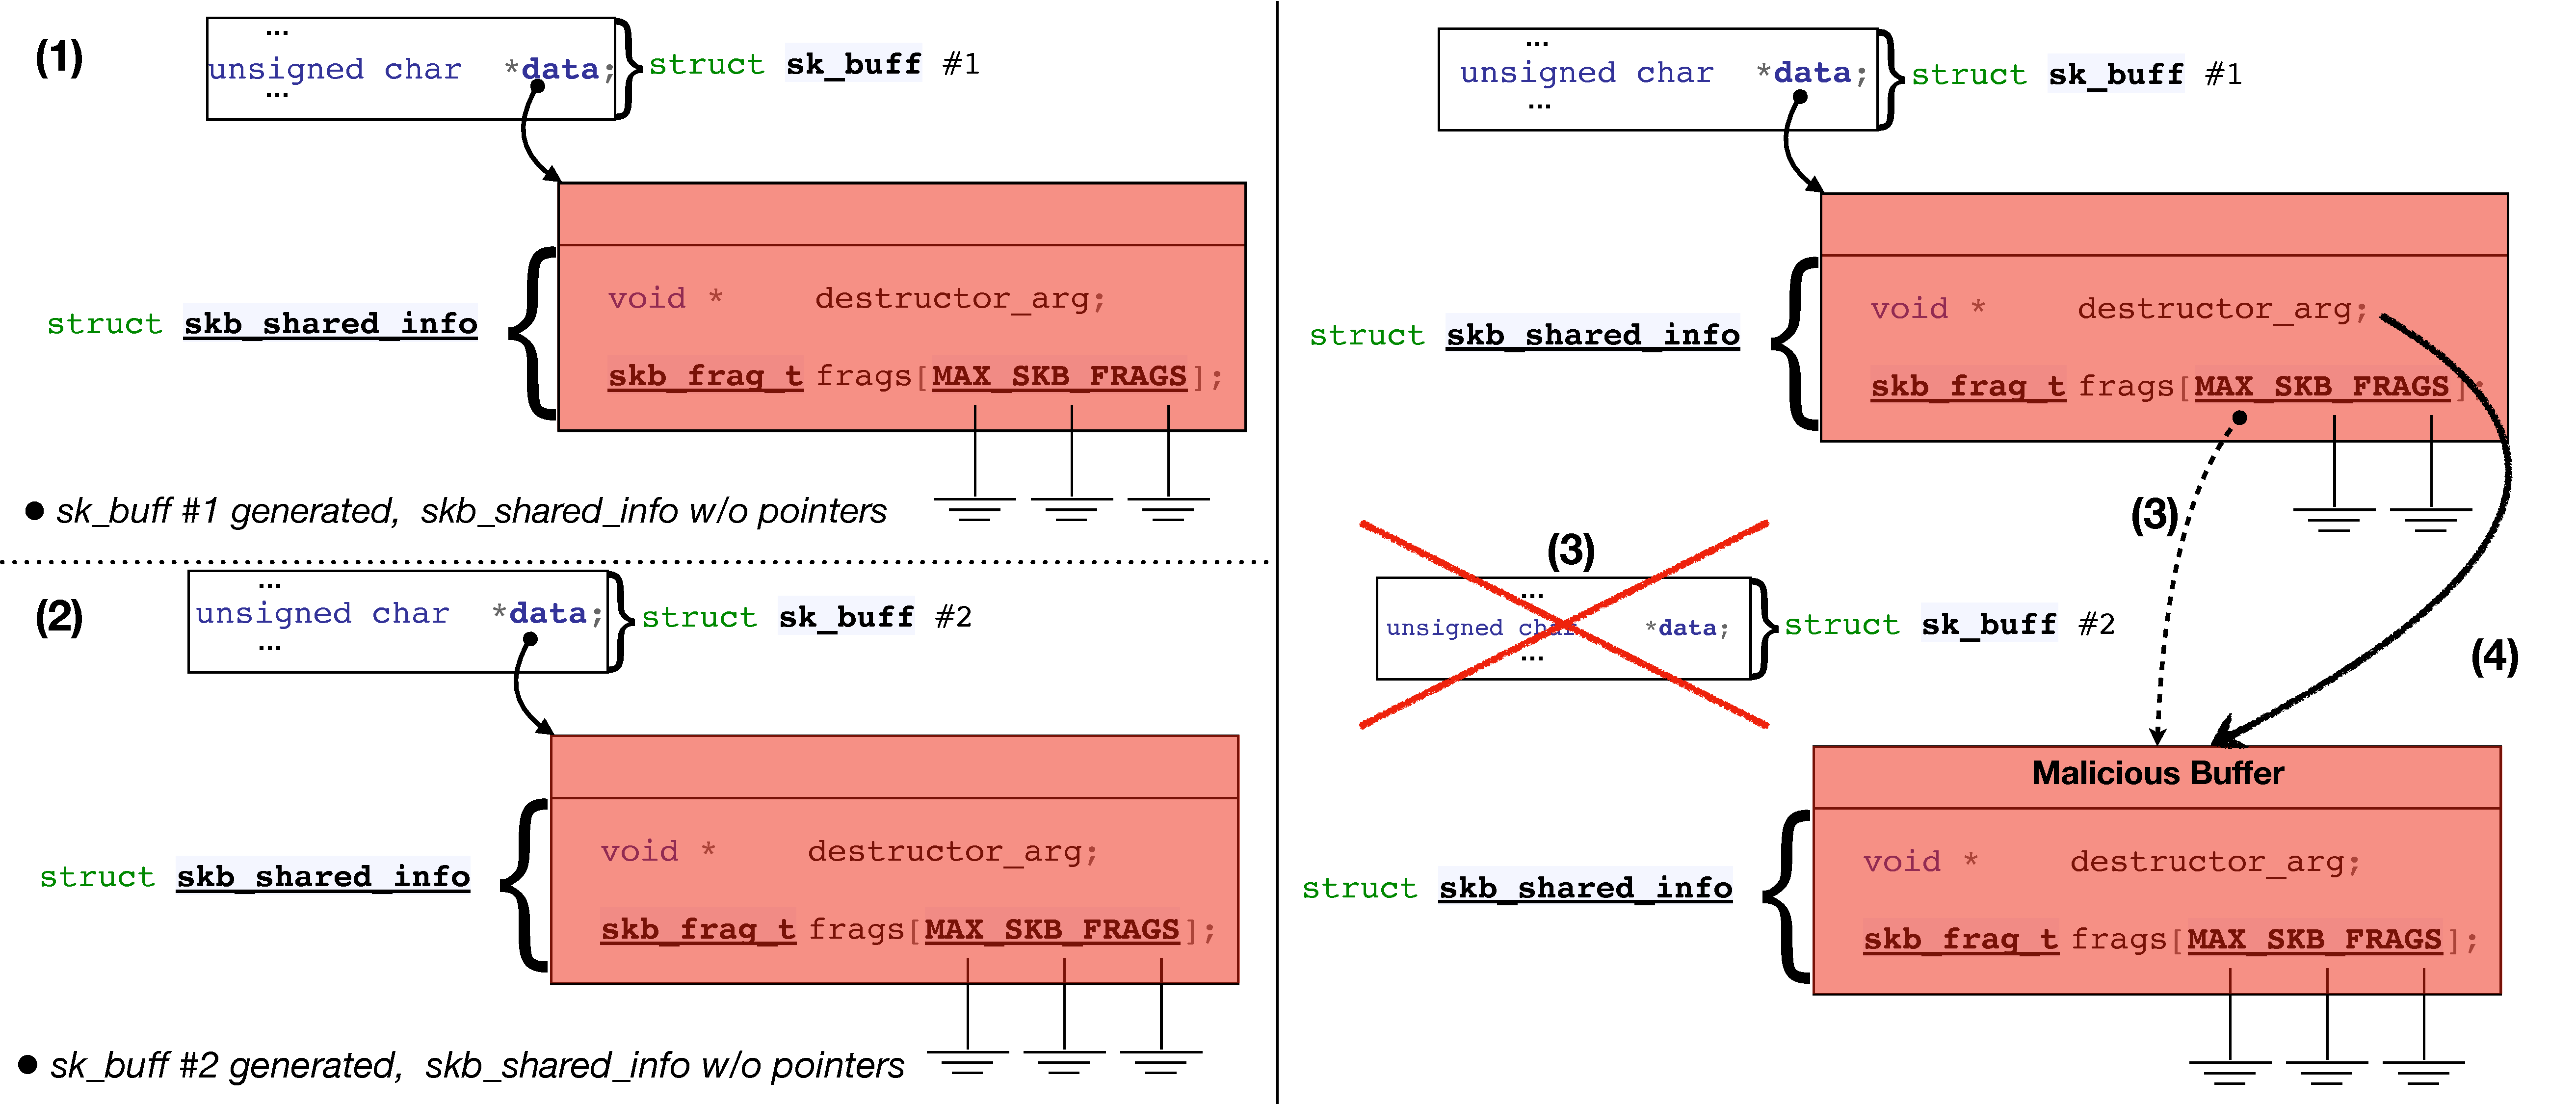
\includegraphics[width=\linewidth]{figs/gro.pdf}
    \caption{An RX sk\_buff after GRO, used as a \means for a DMA attack}
    \label{fig:gro}
\end{figure*}

\subsection{XDP}\label{sec:xdp}
XDP\footnote{\url{https://www.iovisor.org/technology/xdp}} provides a way for users to add custom handling to RX buffers with little overhead. Use cases, include DDOs mitigation for security and Forwarding and load balancing; for the latter the RX buffers need to be also readable to the NIC. As a result all RX buffers are mapped with DMA\_BIDIRECTIONAL rather than the usual DMA\_FROM device. Additionally, in an attempt to avoid performance penalties from memory allocation \cite{xdp} and DMA mapping/unmapping; the RX buffers are reused in a page\_pool\cite{page_pool}. These, pages are never unmapped, and remain accessible to the device both for read and write through out the pools existence (read forever). In this section we will focus on the latest mlx5\_core drivers of the NICs we have on our setup. Other drivers with XDP patches show similar behaviour\footnote{\textcolor{red}{Add a list of drivers to Appendix}}. It is important to note, that a DMA-page pool mechanism is not an inherently bad idea when implemented with caution\cite{MSMT18}. Also, its important to note that the mlx5\_core driver has two modes of operation; linear - where an skb is built around an RX buffer and non-linear where the driver is is filling up the \texttt{frags} of \shinfo. The former is the default, and the later is actually secure. The non-linear mode of option is secure because \shinfo is never accessible to the device; and thus the NIC never has the \oportunity to attack.\newline
In linear mode the NIC has both read, and write access to \shinfo; this additional read capability allows the NIC to run and exploit in 4 steps (Fig \ref{fig:gro}):
\begin{enumerate}
    \item An RX \skb is generated, its part of a TCP stream. \shinfo is initialised by the CPU and the \texttt{frags} are filled with NULL pointers.
    \item A second RX \skb is generated and its part of the same TCP stream.
    \item The second \skb is coalesced with the first packet. The \skb is freed and the \data is added as a \texttt{frag} to the first \skb.
    \item The NIC reads the updated \texttt{frag} field, translates the \page address to a valid \kva and finally fills the \texttt{destructor\_arg} field. Creating a poisoned \skb like in Fig \ref{fig:sh_info}.
\end{enumerate}
The difference between this flow and a regular receive flow is the additional read capability the NIC has due to XDP.
\textcolor{magenta}{\subsection{ICMP}
In the ICMP code I have noticed; what seems to be a reuse of RX skbs for TX, resulting in READ/WRITE mapping - this can allow the device to read all server memory. Unfortunately privilege escalation is infeasible due to lack of \means, until of-course we find a scenario where ICMP adds, write accessible frags.} 

\begin{comment}
%The linear skbs in mlx5 are mapping sh\_info as BI\_DIR, need to see when linear used vs non-linear and to check othe XDP drivers. When sh\_info is mapped BI\_DIR its all we need to attack.\newline It seems linear skb (No (HW?)LRO and MTU<1500 : verify with experimnt or Boris) means no frags, while \begin{enumerate}
%    \item build\_skb is used on a mapped page
%    \item page is unmapped in a deferred way, regardless of iommu policy; a driver hack.
%\end{enumerate} 
 \begin{enumerate}
    \item skb\_try\_coalesce
    \item SW LRO/GRO
\end{enumerate}.
\newline
\textcolor{magenta}{In addition reviewing other drivers for the intersection of DMA\_BIDIR \^ (skb\_add\_rx\_frag||skb\_fill\_page\_descriptor)}
\end{comment}
